% !TeX root = ../document.tex

\chapter{狭义相对论}
\begin{xiti}
	\item 惯性 观者$G$和$G^\prime$相对 速率 为$u=0.6 c$,相遇 时 把 时钟 都 调为 零。用 时空图 讨论:(a) 在$G$所属的惯性参考系看来(以其同时观判断),当$G$钟读数为$\SI{5}{\micro\second} $时,$G^\prime$钟的读数是多少?(b)当$G$钟读数为$\SI{5}{\micro\second} $时,他实际看见$G^\prime$钟的读数是多少?
	
	\begin{jie}
		如图~\ref{pic-6.1},其中$a$点$G$的固有时为$\tau=\SI{5}{\micro\second}$。
		
		\begin{figure}[htb!]
			\centering
			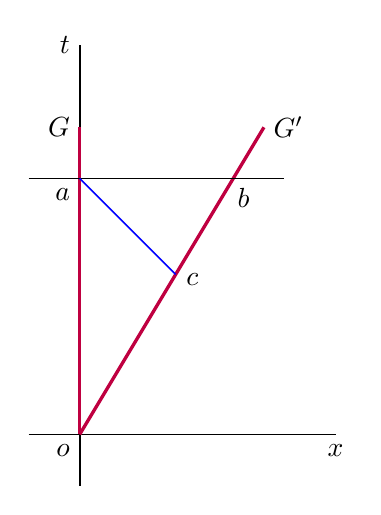
\begin{tikzpicture}[scale=1.3]
			\node[below] (x) at (2.5,0) {$x$};
			\node[left] (t) at (0,3.8) {$t$};
			\node[below left] (O) at (0,0) {$o$};
			\node[left] (G) at (0,3) {$G$};
			\node[right] (g) at (1.8,3) {$G^\prime$};
			\node[below left] (tau) at (0,2.5) {$a$};
			\node[below] (b) at (1.6,2.5) {$b$};
			\node[below] (c) at (1.1,1.6625) {$c$};
			\draw[semithick,\myarrow] (-0.5,0) -- (2.5,0);
			\draw[semithick,\myarrow] (0,-0.5) -- (0,3.8);
			\draw[very thick,purple] (0,0) -- (0,3);
			\draw[very thick,purple] (0,0) -- (1.8,3);
			\draw (-0.5,2.5) -- (2,2.5);
			\draw[semithick,blue,\myarrow] (0.938,1.562) -- (0,2.5);
			\end{tikzpicture}
			\caption{题1解答图}\label{pic-6.1}
		\end{figure}
	
	    \begin{enumerate}
	    	\item[(a)] 易知 $b$点的$x$坐标为$0.6\tau$,于是 $b$ 点 $G^\prime$ 的固有时为 \[\tau^\prime = \sqrt{1-0.6^2} \tau = 0.8 \tau = \SI{4}{\micro\second}.\]
	    	\item[(b)] 易求得$b$点在${t,x}$坐标系下的坐标为 $\displaystyle \left( \frac{3}{8} \tau ,\frac{5}{8} \tau \right)$,于是$c$点$G'$的固有时为 \[ \tau^{\prime\prime} = \sqrt{\left(\frac{5}{8}\right)^2-\left(\frac{3}{8}\right)^2} \tau = \frac{\tau}{2} = \SI{2.5}{\micro\second}. \]
	    \end{enumerate}
	\end{jie}
	
	\item 远方星体以$0.8 c $的速率(匀速直线地)离开我们,我们测得它辐射来的闪光按$5$昼夜的周期变化。用时空图求星上观者测得的闪光周期。
	
	\begin{jie}
		如图~\ref{pic-6.2},
		\begin{figure}[htb!]
			\centering
			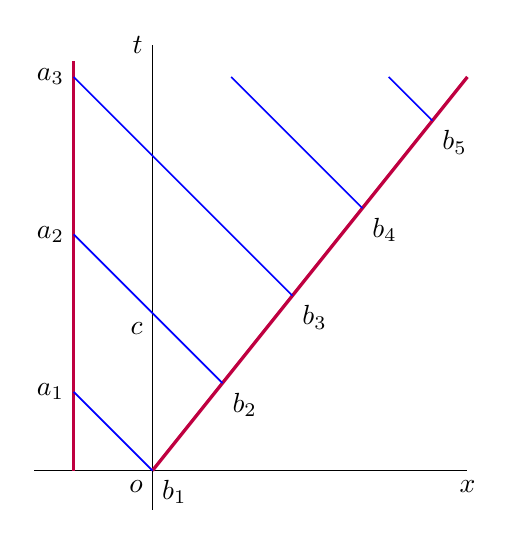
\begin{tikzpicture}
			\node[below] (x) at (5,0) {$x$};
			\node[left] (t) at (1,5.4) {$t$};
			\node[below left] (O) at (1,0) {$o$};
			\node[left] (a1) at (0,1) {$a_1$};
			\node[left] (a2) at (0,3) {$a_2$};
			\node[left] (a3) at (0,5) {$a_3$};
			\node[below right] (b1) at (1,0) {$b_1$};
			\node[below left] (c) at (1,2) {$c$};
			\draw[semithick,\myarrow] (-0.5,0) -- (5,0);
			\draw[semithick,\myarrow] (1,-0.5) -- (1,5.4);
			\draw[very thick,purple] (0,0) -- (0,5.2);
			\draw[very thick,purple] (1,0) -- (5,5);
			\draw[semithick,blue,\myarrow] (1.8889,1.1111) node[below right,black] {$b_2$} -- (0,3);
			\draw[semithick,blue,\myarrow] (1,0) -- (0,1);
			\draw[semithick,blue,\myarrow] (2.7778,2.2222) node[below right,black] {$b_3$} -- (0,5);
			\draw[semithick,blue,\myarrow] (3.6667,3.3333) node[below right,black] {$b_4$} -- (2,5);
			\draw[semithick,blue,\myarrow] (4.5556,4.4444) node[below right,black] {$b_5$} -- (4,5);
			\end{tikzpicture}
			\caption{题2解答图}\label{pic-6.2}
		\end{figure}
	    记$c$点坐标为$\left(0,\tau\right)$,其中$\tau=\SI{5}{\day}$,则可算得$b_2$点坐标为 $\displaystyle \left(\frac{4}{9},\frac{5}{9}\right) \tau$,于是$b_1$到$b_2$星上观者经过的固有时$\displaystyle \tau^{\prime} = \sqrt{5^2-4^2} \frac{\tau}{9} = \frac{\tau}{3} = \frac{5}{3} \,\si{\day}.$
	\end{jie}
	
	\item 把图~\hyperlink{6-20}{6-20}~的 $oa$ 段和 $oe$ 段线长分别记作 $\tau$ 和 $\tau^\prime$ 。(a) 用两钟的相对速率 $u$ 表出 $\tau^\prime/\tau$ ;(b) 在 $u=0.6c$ 和 $u=0.8c$ 两种情况下求出 $\tau^\prime/\tau$ 的数值。
	
	\begin{figure}[htb!]
		\centering
		\begin{tikzpicture}
		\draw[very thick,purple] (0,0) node[left,black] {$o$} -- (0,-5);
		\draw[very thick,purple] (0,0) -- (2,-5);
		\node[above left] (a) at (0,-2) {$a$};
		\draw[semithick,domain=-1.732:1.732,variable=\t,range=0:4, smooth] plot ({2*\t},{-2*sqrt(\t*\t+1)});
		\draw[semithick,blue,\myarrow] (1.333,-3.333) node[below right,black] {$e$} -- (0,-2);
		\node (jz) at (-2.15,-3) {\colorbox{white}{校准曲线}};
		\node[above,rotate=90] (c) at (0,-3.5) {$C$钟(观者$G$)};
		\node (cc) at (1,-0.9) {$C'$钟};
		\end{tikzpicture}
		\caption{正文图6-20}\hypertarget{6-20}{}
	\end{figure}
    
    \begin{jie}
    	\begin{enumerate}
    		\item[(a)] 如图~\ref{pic-6.3},记 $t=of$,
    		\begin{equation}
    		\frac{\tau'}{\tau} = \frac{\sqrt{t^2-u^2 t^2}}{t-ut} = \sqrt{\frac{1+u}{1-u}}.
    		\end{equation}
    		
    		\begin{figure}[htb!]
    			\centering
    			\begin{tikzpicture}
    			\draw[very thick,purple] (0,0) node[left,black] {$o$} -- (0,-5);
    			\draw[very thick,purple] (0,0) -- (2,-5);
    			\node[above left] (a) at (0,-2) {$a$};
    			\draw[semithick,domain=-1.732:1.732,variable=\t,range=0:4, smooth] plot ({2*\t},{-2*sqrt(\t*\t+1)});
    			\draw[semithick,blue,\myarrow] (1.333,-3.333) node[below right,black] {$e$} -- (0,-2);
    			\draw[semithick] (1.333,-3.333) -- (0,-3.333) node[below right] {$f$} ;
    			\node (jz) at (-2.15,-3) {\colorbox{white}{校准曲线}};
    			\node[above,rotate=90] (c) at (0,-3.5) {$C$钟(观者$G$)};
    			\node (cc) at (1,-0.9) {$C'$钟};
    			\end{tikzpicture}
    			\caption{题3解答图}\label{pic-6.3}
    		\end{figure}
    	
    	    \item[(b)] 将 $u=0.6$ 和 $u=0.8$ 代入,分别得 $\dfrac{\tau'}{\tau}$ 为 $2$ 和 $3$。
    	\end{enumerate}
    \end{jie}
    
    \item 惯性质点 $A,B,C$ 排成一条直线并沿此线相对运动(见~\hyperlink{t5}{图 6.5}),相对速率 $u_{BA}=0.6 c$ , $u_{CA}=0.8 c$ ,$A,B$ 所在惯性系各为 $\mathscr{R}_A$ 和 $\mathscr{R}_B$。设 $\mathscr{R}_B$ 系认为(测得)$C$ 走了 $\SI{60}{m}$,画出时空图并求 $\mathscr{R}_A$ 认为(测得)这一过程的时间。
    
    \begin{figure}[htb!]
    	\centering
    	\begin{tikzpicture}[scale=1.5]
    	\filldraw (0,0) circle (0.02cm);
    	\filldraw (1,0) circle (0.02cm);
    	\filldraw (2,0) circle (0.02cm);
    	\draw[semithick] (0,0) node[below] {$A$} -- (1,0) node[below] {$B$} -- (2,0) node[below] {$C$} -- (3,0);
    	\draw[thick,-{Latex[length=6pt,width'=0pt 0.4]}] (1,0.15) -- (1.6,0.15);
    	\draw[thick,-{Latex[length=6pt,width'=0pt 0.4]}] (2,0.15) -- (2.8,0.15);
    	\end{tikzpicture}
    	\caption{题4用图}\hypertarget{t5}{}
    \end{figure}
    
    \begin{jie}
    	如图~\ref{pic-6.4},
    	\begin{figure}[htb!]
    		\centering
    		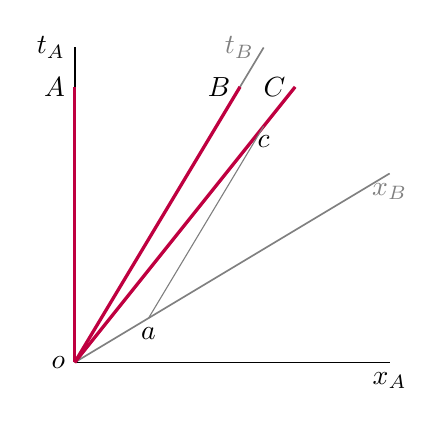
\begin{tikzpicture}
    		\draw[semithick,\myarrow] (0,0) -- (4,0);
			\draw[semithick,\myarrow] (0,0) -- (0,4);
			\draw[semithick,gray,\myarrow] (0,0) -- (2.4,4);
			\draw[semithick,gray,\myarrow] (0,0) -- (4,2.4);
			\node[left] (o) at (0,0) {$o$};
			\node[left] (tA) at (0,4) {$t_A$};
			\node[below] (xA) at (4,0) {$x_A$};
			\node[left,gray] (tB) at (2.4,4) {$t_B$};
			\node[below,gray] (xB) at (4,2.4) {$x_B$};
    		\draw[very thick,purple] (0,0) -- (0,3.5);
    		\draw[very thick,purple] (0,0) -- (2.1,3.5);
			\draw[very thick,purple] (0,0) -- (2.8,3.5);
			\node[left] (A) at (0,3.5) {$A$};
			\node[left] (B) at (2.1,3.5) {$B$};
			\node[left] (C) at (2.8,3.5) {$C$};
			\draw[gray] (0.9375,0.5625) -- (2.4,3);
			\node[below] (c) at (2.4,3) {$c$};
			\node[below] (D) at (0.9375,0.5625) {$a$};
			\end{tikzpicture}
			\caption{题4解答图}\label{pic-6.4}
		\end{figure}
		$oa$ 段长 $\displaystyle l=\SI{60}{\meter}$,则可算得 $a$ 的坐标为 $\displaystyle \left( \frac{5}{4} , \frac{3}{4} \right) l$,由 $ac$ 的斜率为 $\displaystyle \frac{1}{0.6 c}$,$oc$ 的斜率为 $\displaystyle \frac{1}{0.8c}$ 可求得 $c$ 点坐标为 $\displaystyle \left(\frac{16}{5},\frac{4}{c} \right) l$,即 $oc$ 在 $\mathscr{R}_A$ 看来的时间为 $\displaystyle \frac{4l}{c} = \frac{240}{299792458} \si{\second}$。
	\end{jie}
	
	\item $A,B$ 是同一惯性系的两个惯性观者,他们互相发射中子,每一中子以相对速率 $0.6 c$ 离开中子枪。设 $B$ 测得 $B$ 枪的中子发射速率为 $\SI{e4}{s^{-1}}$ (即每秒发射 $10^4$ 个),求 $A$ 所发中子(根据中子自己的标准钟)测得的 $B$ 枪的中子发射率(要求画时空图求解)。
	
	\begin{jie}
		如图~\ref{pic-6.5},$oa$长为 $\Delta\tau_B$,则由对称性易知 $ob=ab=\frac{\Delta\tau_B}{2}$,则 $bc=0.3\Delta\tau_B$,故算得 $\Delta\tau=ac=0.4\Delta\tau_B$,因此 $A$ 发射的中子测得的 $B$ 的发射率为 $f=\frac{1}{\Delta\tau}=2.5f_B=\SI{2.5e4}{\per\second}$。
		\begin{figure}[htb!]
			\centering
			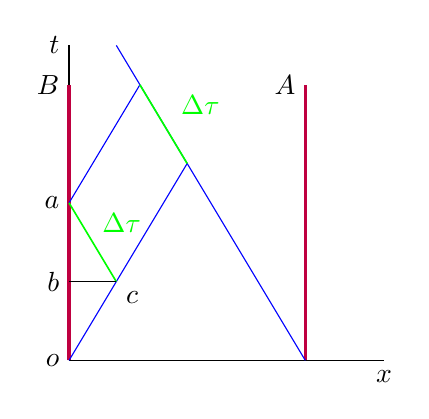
\begin{tikzpicture}
				\draw[semithick,\myarrow] (0,0) -- (0,4);
				\draw[semithick,\myarrow] (0,0) -- (4,0);
				\draw[very thick,purple] (0,0) -- (0,3.5);
				\draw[very thick,purple] (3,0) -- (3,3.5);
				\node[left] (o) at (0,0) {$o$};
				\node[left] (t) at (0,4) {$t$};
				\node[below] (x) at (4,0) {$x$};
				\node[left] (A) at (3,3.5) {$A$};
				\node[left] (B) at (0,3.5) {$B$};
				\draw[blue,\myarrow] (3,0) -- (0.6,4);
				\draw[blue,\myarrow] (0,0) -- (1.5,2.5);
				\draw[blue,\myarrow] (0,2) -- (0.9,3.5);
				\draw[semithick,green] (0.9,3.5) -- (1.5,2.5);
				\draw[semithick,green] (0,2) -- (0.6,1);
				\node[above right,green] (tau) at (1.3,3) {$\Delta \tau$};
				\node[above right,green] (tau2) at (0.3,1.5) {$\Delta \tau$};
				\node[left] (a) at (0,2) {$a$};
				\node[left] (b) at (0,1) {$b$};
				\node[below right] (c) at (0.6,1) {$c$};
				\draw (0,1) -- (0.6,1);
			\end{tikzpicture}
			\caption{题5解答图}\label{pic-6.5}
		\end{figure}
	\end{jie}

	\item 静止 $\mu$ 子的平均寿命为 $\tau_0=\SI{2e-6}{s}$。宇宙线产生的 $\mu$ 子相对于地球以 $0.995c$ 的速率匀速直线下落,用时空图求地球观者测得的(a)$\mu$子的平均寿命;(b)$\mu$子在其平均寿命内所走过的距离。
	
		\begin{jie}
			如图~\ref{pic-6.6},$ac=\tau_0$,$bc=t$ 为地球看来的平均寿命。则 $ab=0.995t$,有
			\begin{equation*}
				\tau_0=ac=\sqrt{\abs{-t^2+(0.995t)^2}}\approx 0.09987 t,
			\end{equation*}
			故 $t\approx 10.0125 \tau_0 = \SI{2.0025e-5}{\second}$,而走过的距离为 $ab=vt\approx\SI{5.9733}{\kilo\metre}$。 
			\begin{figure}[htb!]
				\centering
				\begin{tikzpicture}
					\draw[semithick,\myarrow] (0,0) -- (0,3);
					\draw[semithick,\myarrow] (0,0) -- (4,0);
					\node[left] (o) at (0,0) {$o$};
					\node[left] (t) at (0,3) {$t$};
					\node[below] (x) at (4,0) {$x$};
					\draw[blue,\myarrow] (3,0) -- (1.01,2);
					\draw[very thick,purple] (0,0) -- (0,2.5);
					\draw[gray] (1.01,0) -- (1.01,2);
					\node[below] (a) at (3,0) {$a$};
					\node[below left] (b) at (1.01,0) {$b$};
					\node[left] (c) at (1.01,2) {$c$};
				\end{tikzpicture}
				\caption{图6解答图}\label{pic-6.6}
			\end{figure}
		\end{jie}

	\item 从惯性系 $\mathscr{R}$ 看来(认为,测得),位于某地 $A$ 的两标准钟甲、乙指零时开始以速率 $v=0.6c$ 一同做匀速直线运动,两钟指 $\SI{1}{\second}$ 时到达某地 $B$。甲钟在到达 $B$ 地时立即以速率 $v$ 向 $A$ 地匀速返回,乙钟在 $B$ 地停留 $\SI{1}{\second}$ (按他的钟)后以速率 $v$ 向 $A$ 的匀速返回。另有一丙钟一直呆在 $A$ 地,且当甲、乙离开 $A$ 地时也指零,(a) 画出甲、乙、丙的世界线;(b) 求乙钟返回 $A$ 地时三钟的读数 $\tau_{\text{甲}}$,$\tau_{\text{乙}}$ 和 $\tau_{\text{丙}}$。
	
		\begin{jie}
			如图~\ref{pic-6.7},设$A$ 地位于 $x=0$,$B$ 地位于 $x=s$。
			\begin{figure}[htb!]
				\centering
				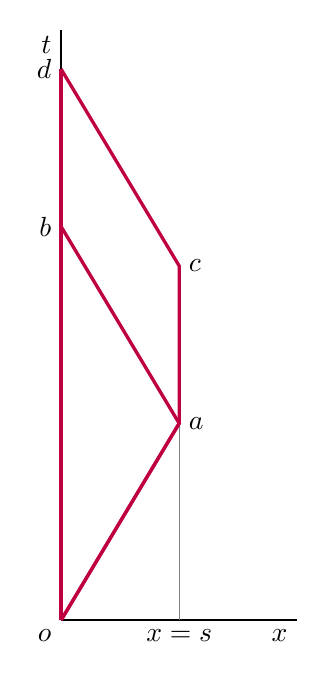
\begin{tikzpicture}
					\draw[semithick,\myarrow] (0,0) -- (0,7.5);
					\draw[semithick,\myarrow] (0,0) -- (3,0);
					\node[below left] (o) at (0,0) {$o$};
					\node[left] (t) at (0,7.3) {$t$};
					\node[below left] (x) at (3,0) {$x$};
					\draw[gray] (1.5,0) -- (1.5,2.5);
					\node[below] (s) at (1.5,0) {$x=s$};
					\draw[very thick,purple] (0,0) -- (1.5,2.5) -- (0,5) -- (0,7);
					\draw[very thick,purple] (0,0) -- (1.5,2.5) -- (1.5,4.5) -- (0,7);
					\draw [very thick,purple] (0,0) -- (0,7);
					\node[right] (a) at (1.5,2.5) {$a$};
					\node[left] (b) at (0,5) {$b$};
					\node[right] (c) at (1.5,4.5) {$c$};
					\node[left] (d) at (0,7) {$d$};
				\end{tikzpicture}
				\caption{题7解答图}\label{pic-6.7}
			\end{figure}
			\begin{enumerate}[label=(\alph*)]
				\item 甲的世界线为 $oabd$;乙的世界线为 $oacd$;丙的世界线为 $obd$。
				\item 由题干知线长 $oa=ac=ab=bd=cd$ 都是 $\tau=\SI{1}{\second}$,故 $\tau_{\text{甲}}=\tau_{\text{乙}}=\SI{3}{\second}$。$a$ 点位于 $(\frac{5}{3}s,s)$,$oa=\frac{4}{3}s$,故 $s=\frac{3}{4}\tau$,则 $ob=2\times \frac{5}{3}s = \frac{5}{2} \tau$,于是 $\tau_{\text{丙}}=\frac{7}{2}\tau=\SI{3.5}{\second}$。
			\end{enumerate}
		\end{jie}

	\item 暂略。

	\item 暂略。

	\item 暂略。

	\item 暂略。

	\item 试证命题 6-3-4.

	\begin{zm}
		命题6-3-4如下
		\begin{yl}{Thm}
			质点世界线上各点的4加速 $\tensor{A}{^a}$ 与 4 速 $\tensor{U}{^a}$ 正交,即 $\tensor{A}{^a} \tensor{U}{_a} = \tensor{\eta}{_a_b} \tensor{A}{^a} \tensor{U}{^b} =0$。
		\end{yl}
		\begin{yl}{Prf}
			\begin{equation*}
				\begin{split}
					\tensor{U}{_a}\tensor{A}{^a} &= \tensor{U}{_a} \tensor{U}{^b} \Partial{b} \tensor{U}{^a} \\
					&= \frac{1}{2} \tensor{U}{^b} \Partial{b} \left( \tensor{U}{_a} \tensor{U}{^a} \right)\\
					&=0.
				\end{split}
			\end{equation*}
		\end{yl}
	\end{zm}

	\item 设观者世界线为 $t\sim x$ 面内的双曲线 $G$ (见\hyperlink{t6}{图 6.7}),图中 $K$ 为已知,$\tensor{A}{^a}$ 为观者的 4 加速,求 $\tensor{A}{^a} \tensor{A}{_a}$(结论是 $\tensor{A}{^a} \tensor{A}{_a}$ 为常数,因此 $G$ 称为匀加速运动观者\footnote{或称 Rindler 观者——笔者注}。请注意这指的是4加速。)

	\begin{figure}[htb]
		\centering
		\begin{tikzpicture}[decoration={brace,amplitude=6},scale=0.7]
			\draw[semithick,\myarrow] (-3.5,0) -- (3.5,0);
			\draw[semithick,\myarrow] (0,-3.5) -- (0,3.5);
			\node[left] (t) at (0,3.5) {$t$};
			\node[below] (x) at (3.5,0) {$x$};
			\draw[semithick,loosely dash dot] (-3,-3) -- (3,3);
			\draw[semithick,loosely dash dot] (-3,3) -- (3,-3);
			\draw[domain=-1.732:1.732,variable=\t,range=0:4, smooth,thick] plot ({1.5*sqrt(\t*\t+1)},{1.5*\t});
			\node (G) at (2.5,1.5) {$G$};
			\node (K) at (0.75,-0.5) {\colorbox{white}{$K$}};
			\draw[decorate] (1.5,0) -- (0,0);
		\end{tikzpicture}
		\caption{习题13用图}\hypertarget{t6}{}
	\end{figure}

	\begin{jie}
		由图知此双曲线的参数为 $a=b=K$ ,可写出双曲线方程为
		\begin{equation*}
			x^2-t^2=K^2,
		\end{equation*}
		两边对固有时求导,
		\begin{gather*}
			2x \dv{x}{\tau} - 2t \dv{t}{\tau} = 0,\\
			\dv{x}{\tau} = \frac{t}{x} \dv{t}{\tau},
		\end{gather*}
		而
		\begin{equation*}
			\begin{split}
				\tensor{Z}{^a} &= \dv{t}{\tau} \tensor{\left(\pdv{t}\right)}{^a} + \dv{x}{\tau} \tensor{\left(\pdv{x}\right)}{^a}
			\end{split}
		\end{equation*}
		是归一的,则
		\begin{equation*}
			\begin{split}
				\left(\dv{x}{\tau} \right)^2 - \left( \dv{t}{\tau} \right)^2 &= \left[ \left(\frac{t}{x}\right)^2 - 1 \right] \left( \dv{t}{\tau} \right)^2\\
				&= - \left( \frac{K}{x} \dv{t}{\tau} \right)^2\\
				&= -1,
			\end{split}
		\end{equation*}
		\begin{equation*}
			\implies \frac{1}{x} \dv{t}{\tau} = \frac{1}{t} \dv{x}{\tau} = \frac{1}{K},
		\end{equation*}
		于是4速又可改写为
		\begin{equation*}
			\tensor{Z}{^a} = \frac{1}{K} \left[ x \tensor{\left(\pdv{t}\right)}{^a} + t \tensor{\left(\pdv{x}\right)}{^a} \right],
		\end{equation*}
		故
		\begin{equation*}
			\begin{split}
				\tensor{A}{^a} &= \dv{\tensor{Z}{^a}}{\tau}\\
				&= \frac{1}{K} \left[ \dv{x}{\tau} \tensor{\left(\pdv{t}\right)}{^a} + \dv{t}{\tau} \tensor{\left(\pdv{x}\right)}{^a} \right]\\
				&= \frac{1}{K^2} \left[ t \tensor{\left(\pdv{t}\right)}{^a} + x \tensor{\left(\pdv{x}\right)}{^a} \right],\\
				\tensor{A}{_a} \tensor{A}{^a} &= \frac{1}{K^4} \left( x^2 - t^2 \right)\\
				&= \frac{1}{K^2}.
			\end{split}
		\end{equation*}
	\end{jie}

	\item 试证命题6-6-2.

	\begin{zm}
		命题6-6-2如下
		\begin{yl}{Thm}
			设惯性系 $\mathscr{R}$ 和 $\mathscr{R}^\prime$ 由洛伦兹变换
			\begin{equation*}
				t = \gamma \left( t^\prime + v x^\prime \right) \qc x = \gamma \left( x^\prime + v t^\prime \right) \qc y = y^\prime \qc z = z^\prime
			\end{equation*}
			相联系,则两者测同一电磁场 $\tensor{F}{_a_b}$ 所得值 $\left( \myvec{E},\myvec{B} \right)$ 和 $\left( \myvec{E}^\prime , \myvec{B}^\prime \right)$ 有如下关系:
			\begin{align*}
				E_1^\prime &= E_1, & E_2^\prime &= \gamma \left( E_2 - v B_3 \right), & E_3^\prime &= \gamma \left( E_3 + v B_2 \right);\\
				B_1^\prime &= B_1, & B_2^\prime &= \gamma \left( B_2 + v E_3 \right), & B_3^\prime &= \gamma \left( B_3 - v E_2 \right).
			\end{align*}
		\end{yl}
		\begin{yl}{Prf}
			记矩阵 $\Lambda$ 为
			\begin{equation*}
				\left[ \tensor{\Lambda}{^\mu_\nu} \right] = \left[ \pdv{x^\mu}{x^{\prime\nu}} \right] = \mqty( \mqty{ \gamma & \gamma v \\ \gamma v & \gamma }  & \mqty{\zmat{2}{2}} \\ \mqty{\zmat{2}{2}} & \mqty{\imat{2}} ),
			\end{equation*}
			则易知
			\begin{equation*}
				\left[ \tensor{\left(\Lambda^{-1}\right)}{^\mu_\nu} \right] = \left[ \pdv{x^{\prime\mu}}{x^{\nu}} \right] = \mqty( \mqty{ \gamma & - \gamma v \\ - \gamma v & \gamma }  & \mqty{\zmat{2}{2}} \\ \mqty{\zmat{2}{2}} & \mqty{\imat{2}} ),
			\end{equation*}
			而根据张量变换律
			\begin{equation*}
				\begin{split}
					\tensor{{F^\prime}}{^\mu_\nu} &= \pdv{x^{\prime\mu}}{x^\sigma} \pdv{x^\rho}{x^{\prime\nu}} \tensor{F}{^\sigma_\rho}\\
					&= \tensor{\left(\Lambda^{-1}\right)}{^\mu_\sigma} \tensor{F}{^\sigma_\rho} \tensor{\Lambda}{^\rho_\nu},
				\end{split}
			\end{equation*}
			于是有矩阵等式
			\begin{equation*}
				\left[F^\prime\right] = \Lambda^{-1} \left[F\right] \Lambda,
			\end{equation*}
			其中 $\left[F\right]$ 表示 $\tensor{F}{^\mu_\nu}$ 排成的矩阵
			\begin{equation*}
				\left[F\right] = \mqty( 0 & E_1 & E_2 & E_3 \\ E_1 & 0 & B_3 & -B_2 \\ E_2 & -B_3 & 0 & B_1 \\ E_3 & B_2 & -B_1 & 0 ),
			\end{equation*}
			于是经过简单的矩阵乘法算得
			\begin{equation*}
				\left[ F^\prime \right] = \mqty( 0 & E_1 & \gamma \left( E_2 - v B_3 \right) & \gamma \left( E_3 + v B_2 \right) \\ E_1 & 0 & \gamma \left( B_3 - v E_2 \right) & - \gamma \left( B_2 + v E_3 \right) \\ \gamma \left( E_2 - v B_3 \right) & - \gamma \left( B_3 - v E_2 \right) & 0 & B_1 \\ \gamma \left( E_3 + v B_2 \right) & \gamma \left( B_2 + v E_3 \right) & -B_1 & 0 ),
			\end{equation*}
			可以直接读出
			\begin{align*}
				E_1^\prime &= E_1, & E_2^\prime &= \gamma \left( E_2 - v B_3 \right), & E_3^\prime &= \gamma \left( E_3 + v B_2 \right);\\
				B_1^\prime &= B_1, & B_2^\prime &= \gamma \left( B_2 + v E_3 \right), & B_3^\prime &= \gamma \left( B_3 - v E_2 \right).
			\end{align*}
		\end{yl}
	\end{zm}
	
\end{xiti}